\begin{singlespacing}
\chapter{A search for new phenomena}
\label{chapter:2ljets}
%
\begin{epigraphs}
\qitem{%
An experiment is never a failure solely because it fails to
achieve predicted results. An experiment is a failure only when it also
fails adequately to test the hypothesis in question, when the data it
produces don’t prove anything one way or another.%
}%
{Robert M. Pirsig~\cite{pirsig1999zen}}
\qitem{%
But there is one feature I notice that is generally missing in cargo cult
science. \ldots\
% That is the idea that we all hope you have learned in studying science in
% school--we never say explicitly what this is, but just hope that you catch
% on by all the examples of scientific investigation. It is interesting,
% therefore, to bring it out now and speak of it explicitly.
It's a kind of scientific integrity, a principle of scientific thought that
corresponds to a kind of utter honesty --- a kind of leaning over backwards.%
}%
{Richard Feynman~\cite{feynman1974cargo}}
\end{epigraphs}
\end{singlespacing}


We begin with a quick summary of results from my work on this search project;
the coming section briefly presents the plots and tables which I personally
find first when looking at an \atlas\ search paper.
The the meat of this chapter (or if you prefer, its gory details) follows in
Section~\ref{sec:2ljets_context} onwards.


\subsection{Splash summary}

% begin with physics content and results
The sum of my work presented in this thesis is displayed in
Figure~\ref{fig:2ljets_summary}.
It illustrated the unblinded results in regions of the electroweak part of the
recent \atlas\ search ``for new phenomena in events with two leptons, jets, and
missing transverse momentum''~\cite{atlas2022searches}.
For brevity, I call this search $\twoljets$.

In a large number orthogonal signal regions, no significant excess is observed
above \emph{post-fit} backgrounds.
Indeed there are some significant deficits --- data below the background noise.

Background parts of a \heplikelihood model are illustrated behind data.
To test non-standard (supersymmetric) models against observation, signal
contributions are added on top of those backgrounds.

We use two signal models in the $\twoljets$ electroweak analysis.
One is an MSSM chargino-neutralino model (C1N2) which acts to produce
$\chargino{1}\textrm{--}\neutralino{2}$ pairs, which decay via
$W\rightarrow q\bar q$ and
$Z\rightarrow \ell^\pm \ell^\mp$ respectively..
The other is a GMSB model which, after a variety of initial states produces
$\neutralino{1}\textrm{--}\neutralino{1}$ pairs.
These neutralinos decay,
via Higgs and $Z$ bosons in variable branching fractions,
to final states again containing $\ell^\pm \ell^\mp$ and jet-seeding partons.
Diagrams illustrating these C1N2 and GMSB signal models are shown in
Figure~\ref{fig:2ljets_signal_diagrams}.

Effects of some of these these signals in example signal regions of the
$\twoljets$ electroweak analysis are displayed in
Figure~\ref{fig:2ljets_signal_examples}.

At each parameter point of a signal model, it is added to the background model
and tested against data in the $\mathrm{CLs}$ prescription.
Contours showing which parameters of those signal models are labelled as
excluded are displayed for
C1N2 in Figure~\ref{fig:2ljets_contours_c1n2} and for
GMSB in~\ref{fig:2ljets_contours_gmsb}.

Data in discovery regions are presented and interpreted in
Table~\ref{tab:2ljets_discovery}.


% summary plot

\begin{figure}[tp]
\centering
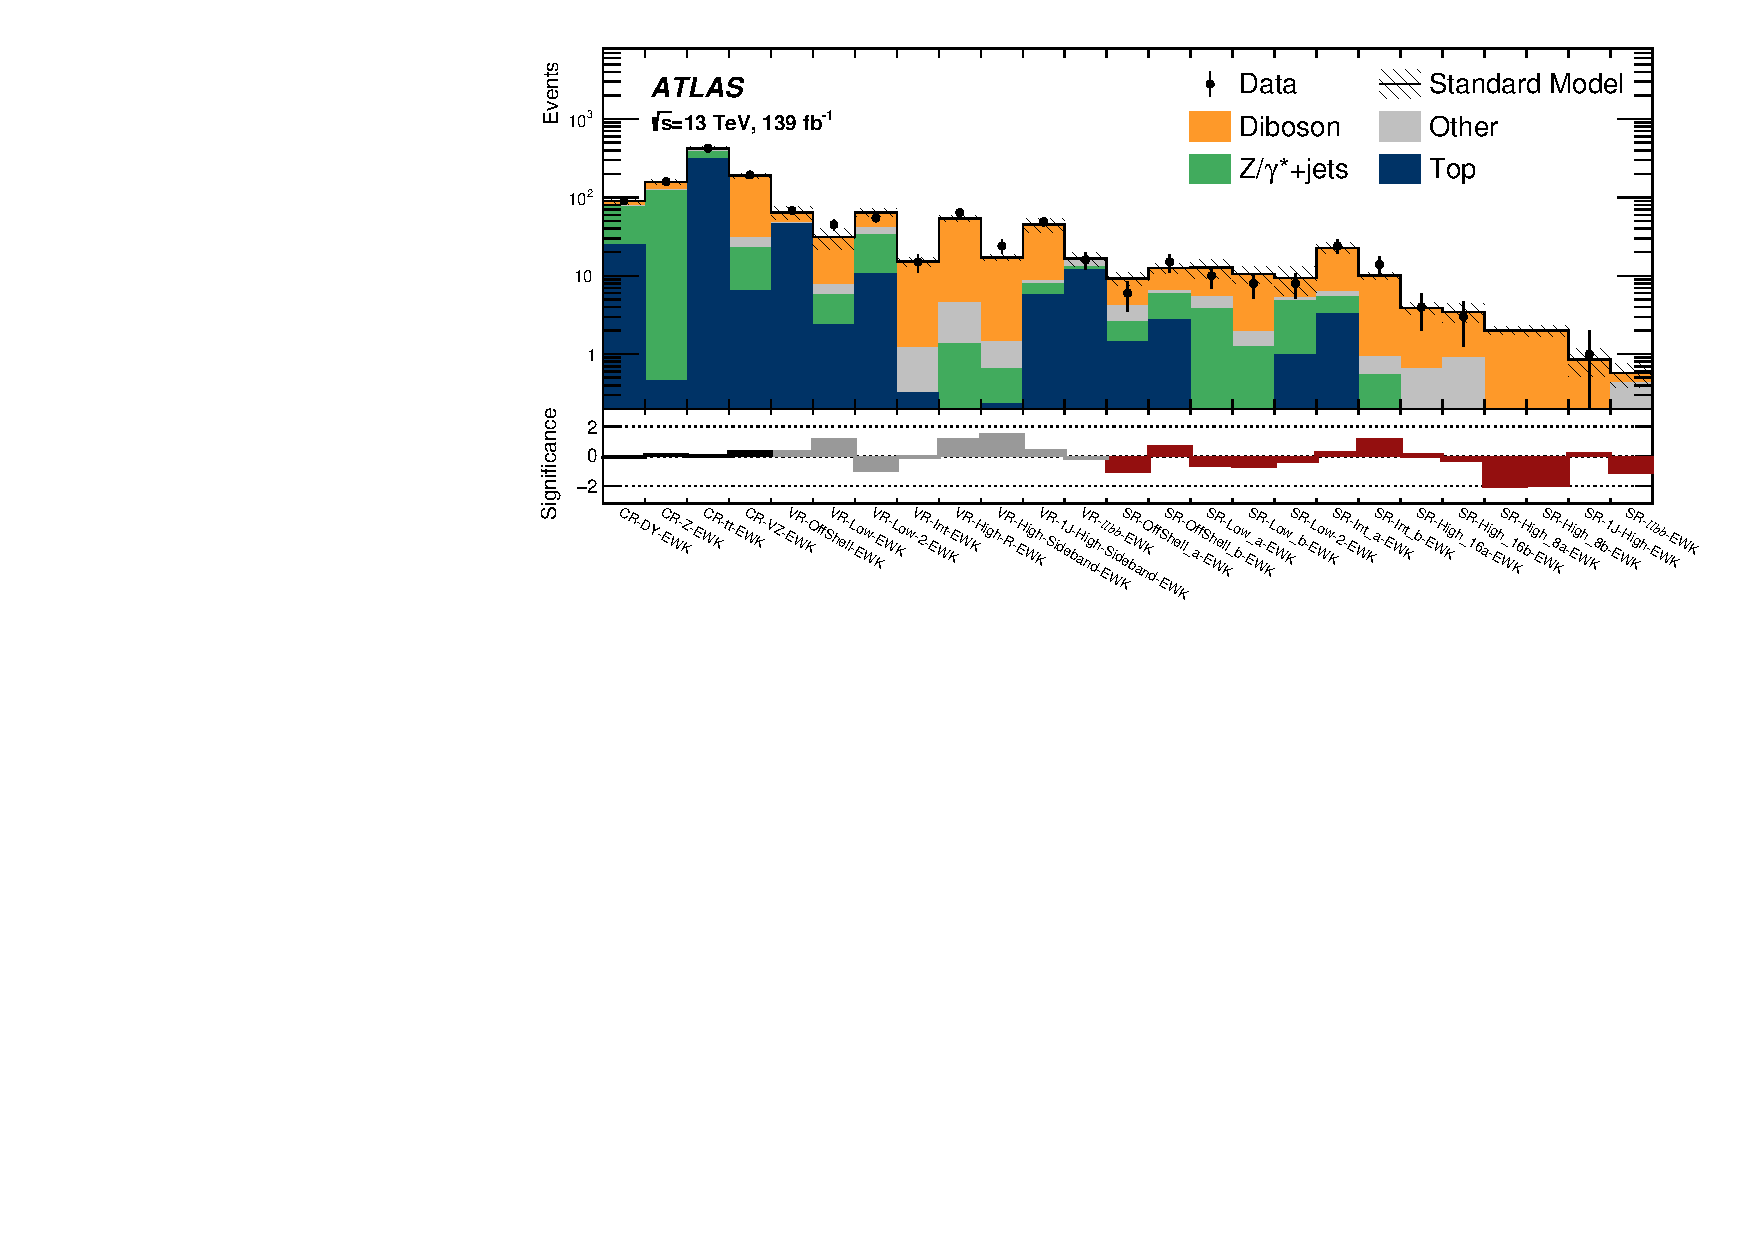
\includegraphics[width=\textwidth]{figures/2ljets_summary_log.pdf}
\caption{%
Data of the $\twoljets$ electroweak analysis with \emph{post-fit}
backgrounds~\cite{atlas2022searches}.
The lower panel shows $S_\mathrm{ATLAS}$ from
Equation~\ref{eqn:significance_atlas}.
Control, validation and signal regions are shown from left to right, with the
regions within each category ordered approximately by their typical $\met$.
Likelihoods from validation regions are not included in the fit.
The `Top' category contains $t\bar t$ and $tW$ processes, and
`Other' contains fake/non-prompt lepton, higgs, triboson, $t\bar tZ$, and other
rare top processes.%
}
\label{fig:2ljets_summary}
\end{figure}


% signal diagrams

\begin{figure}[t]
\centering
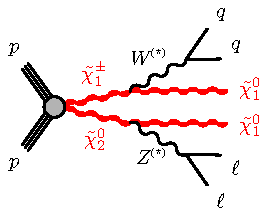
\includegraphics[width=0.48\textwidth]{figures/2ljets_c1n2_llqqn1n1_wz.pdf}
\hfill
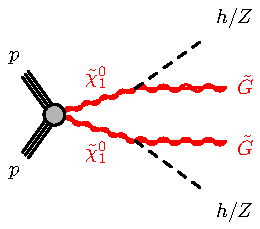
\includegraphics[width=0.45\textwidth]{figures/2ljets_n1n1_hhggzz.pdf}
\caption{%
Supersymmetric signal processes in the $\twoljets$ electroweak
analysis~\cite{atlas2022searches}.
\\[0.5em]
Left: C1N2, where the initial $\chargino{1}\textrm{--}\neutralino{2}$ pair
is produced through a $s$-channel $W^{\pm}$ resonance and the masses of
weak bosons in decays are bounded by the mass splitting
$m(\chargino{1}, \neutralino{2}) - m(\neutralino{1})$.
We explore the parameters
$m(\chargino{1}, \neutralino{2})$ and $m(\neutralino{1})$.
\\[0.5em]
Right: GMSB, where the initial $\neutralino{1}\textrm{--}\neutralino{1}$ pair
is produced by soft decays from pairs including $\chargino{1}$,
$\neutralino{2}$ or $\neutralino{1}$.
Although the $h$ and $Z$ bosons decay to many states, we target
$Z\rightarrow \ell\ell$ with
$h/Z\rightarrow bb/jj$.
We explore the parameters
$m(\neutralino{1})$ and $B(\neutralino{1} \rightarrow h \tilde{G})$ with fixed
$m(\chargino{1}, \neutralino{2}) - m(\neutralino{1}) = 1~\eV[G]$.
}
\label{fig:2ljets_signal_diagrams}
\end{figure}


% signal region plots

\begin{figure}[tp]
\centering
\begin{subfigure}{0.49\textwidth}
    \centering
    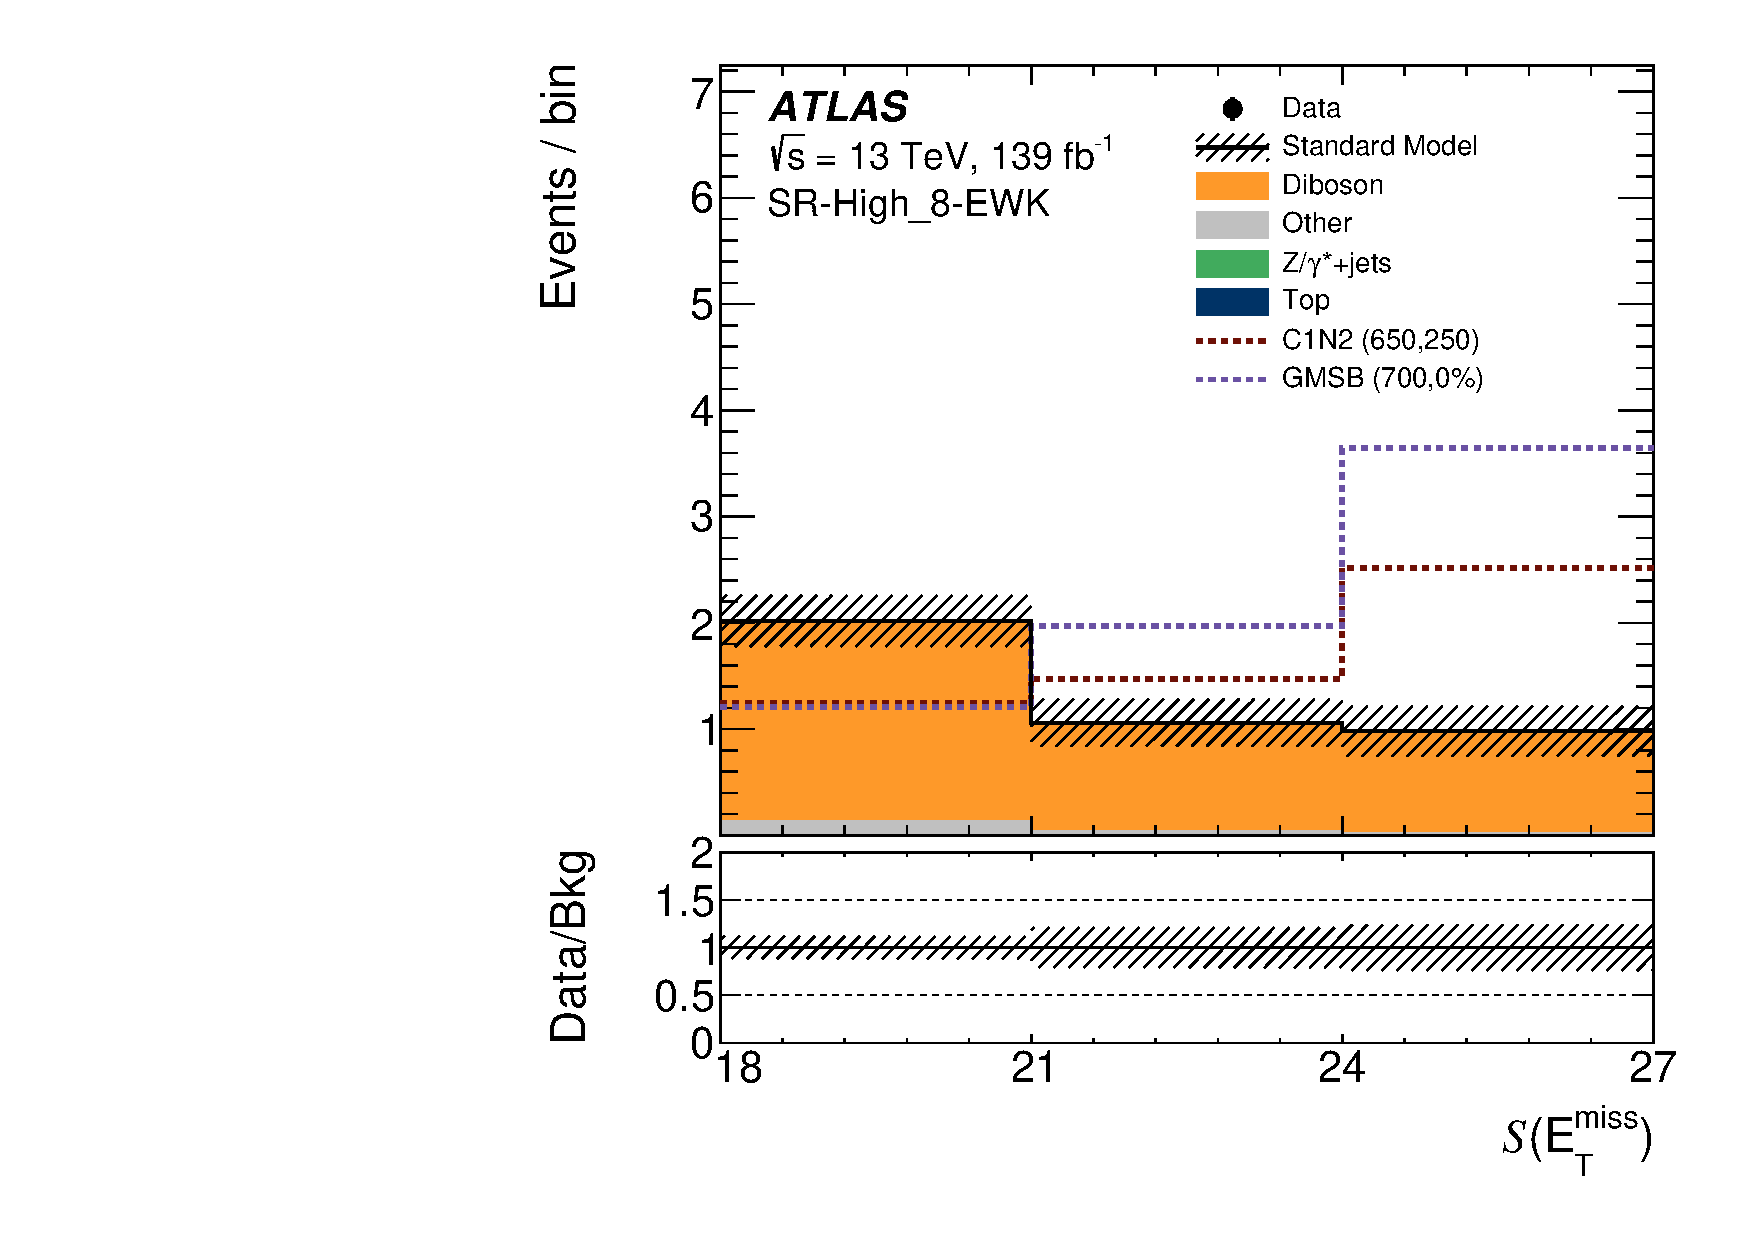
\includegraphics[width=\textwidth]{figures/2ljets_sr_high_8_met_sig.pdf}
    \caption{SR-High-8}
\end{subfigure}
\hfill
\begin{subfigure}{0.49\textwidth}
    \centering
    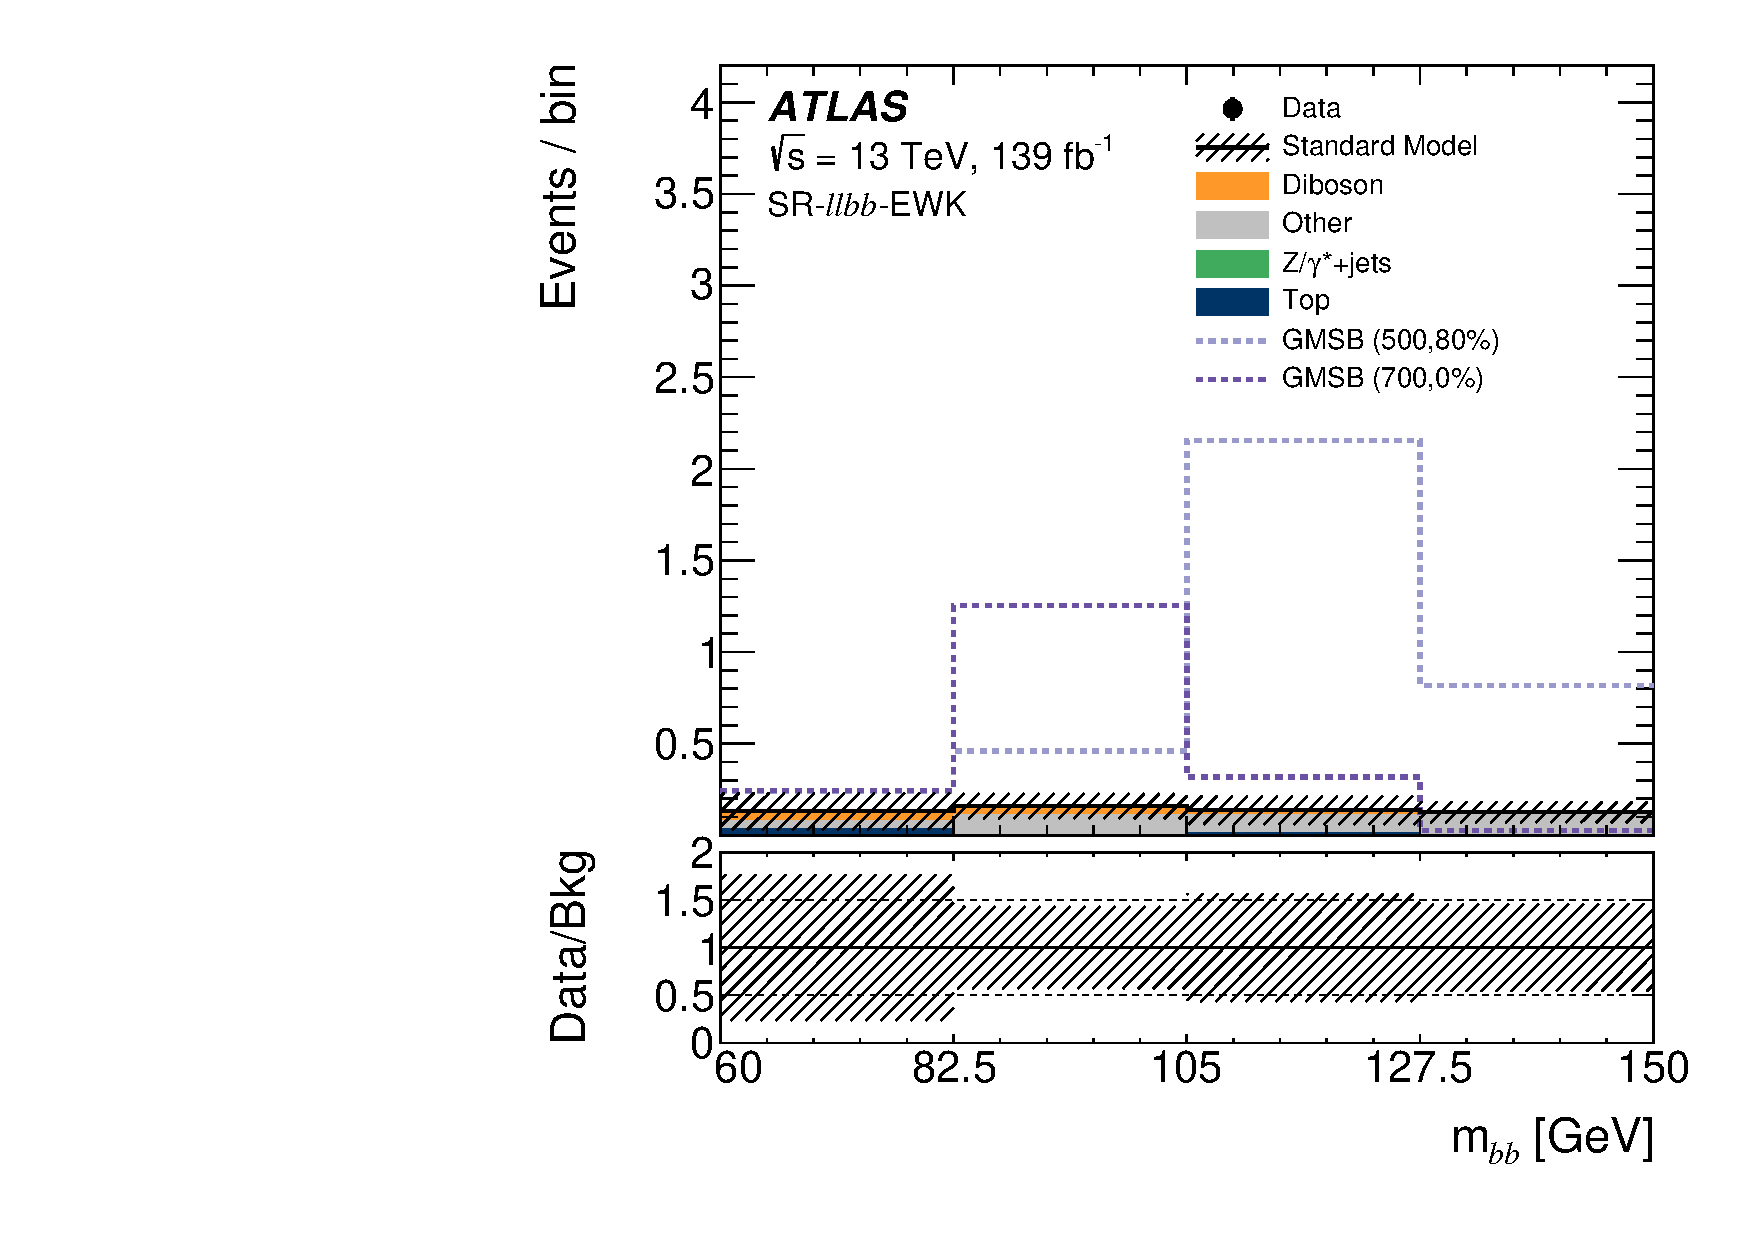
\includegraphics[width=\textwidth]{figures/2ljets_sr_llbb_mbb.pdf}
    \caption{SR-$\ell\ell bb$}
\end{subfigure}
\\[0.5em]
\begin{subfigure}{0.49\textwidth}
    \centering
    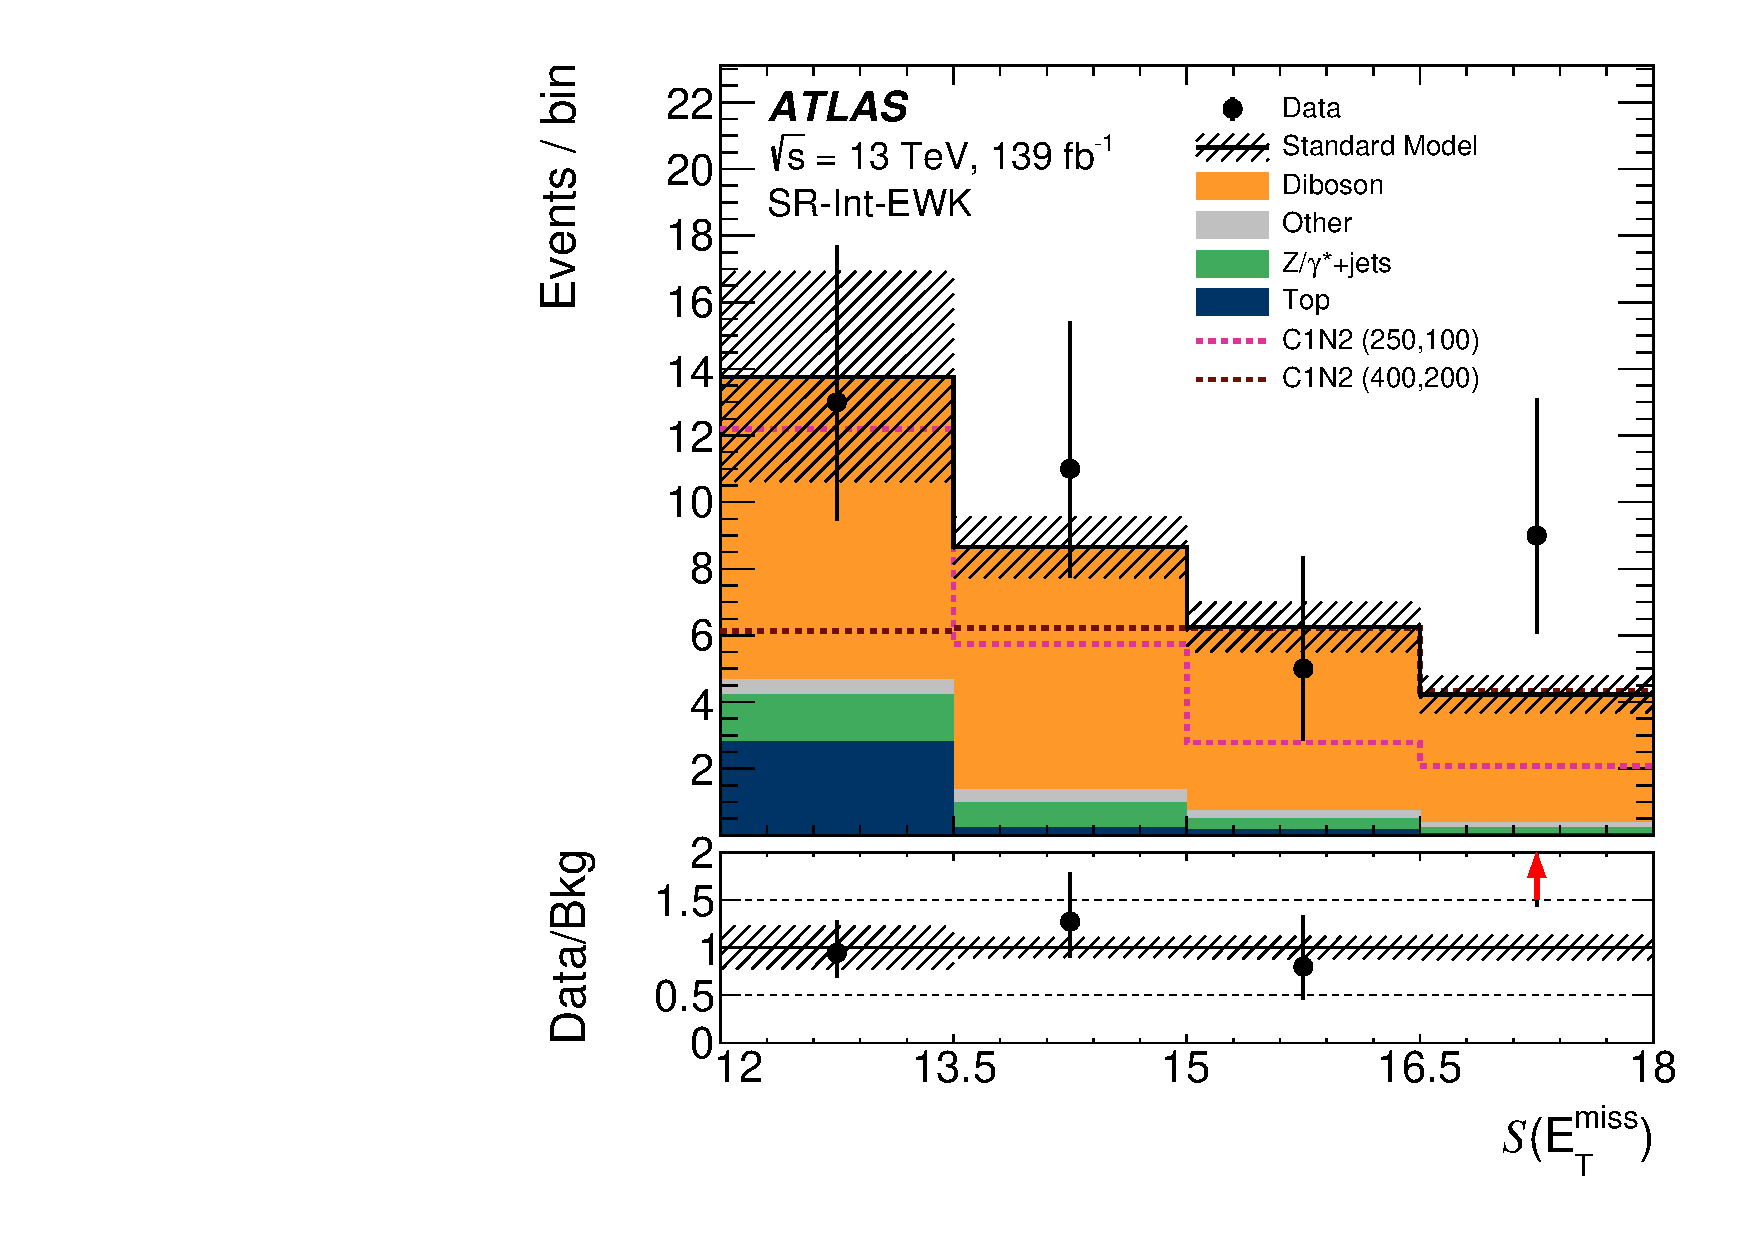
\includegraphics[width=\textwidth]{figures/2ljets_sr_int_met_sig.pdf}
    \caption{SR-Int}
\end{subfigure}
\hfill
\begin{subfigure}{0.49\textwidth}
    \centering
    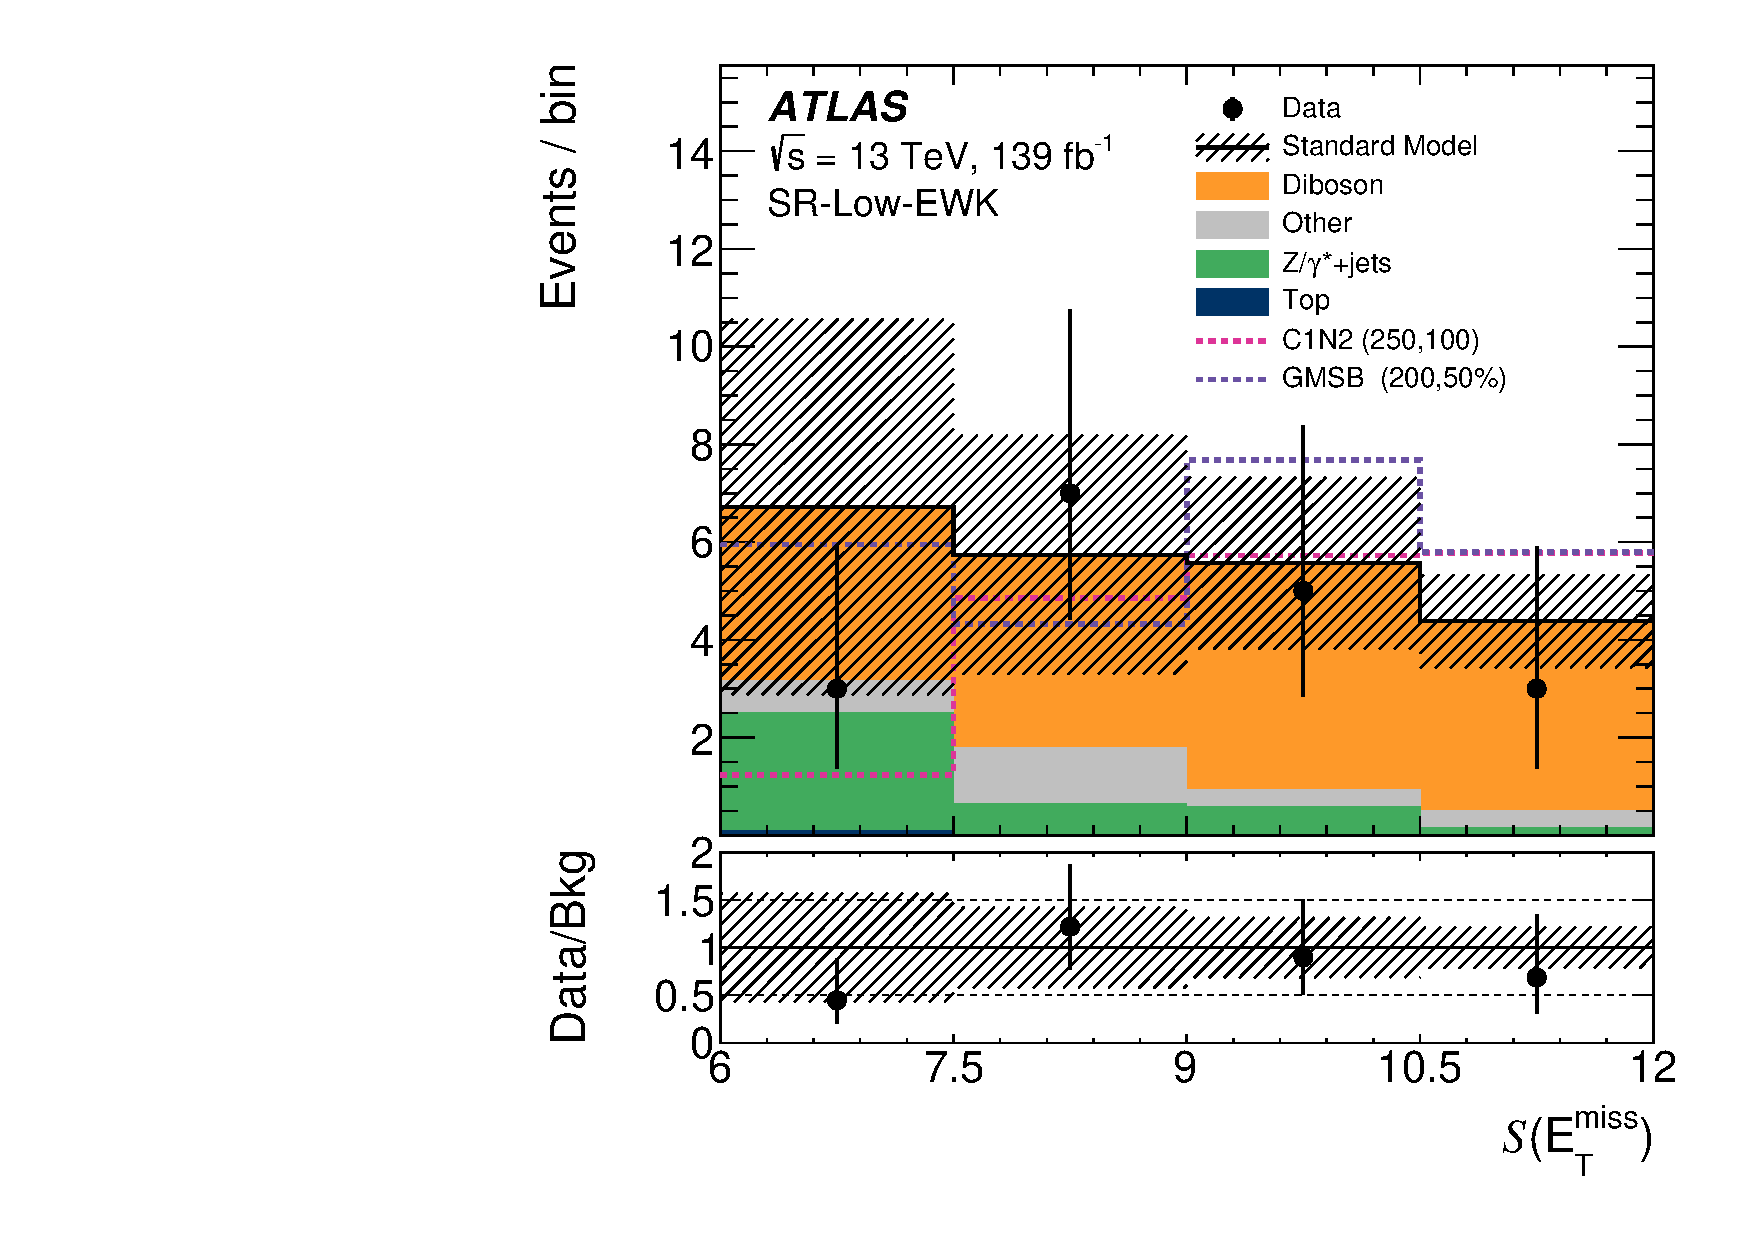
\includegraphics[width=\textwidth]{figures/2ljets_sr_low_met_sig.pdf}
    \caption{SR-Low}
\end{subfigure}
\caption{%
Example signal region histograms with benchmark signal sample yields overlaid
as dotted lines~\cite{atlas2022searches}.
Physically, signal yields would add on top of the backgrounds.
Data are shown; regions in the the top two plots observe zero data, and
Poisson error bars for $0$ events are hidden for aesthetic reasons.
}
\label{fig:2ljets_signal_examples}
\end{figure}



% exclusion plots

\begin{figure}[tp]
\centering
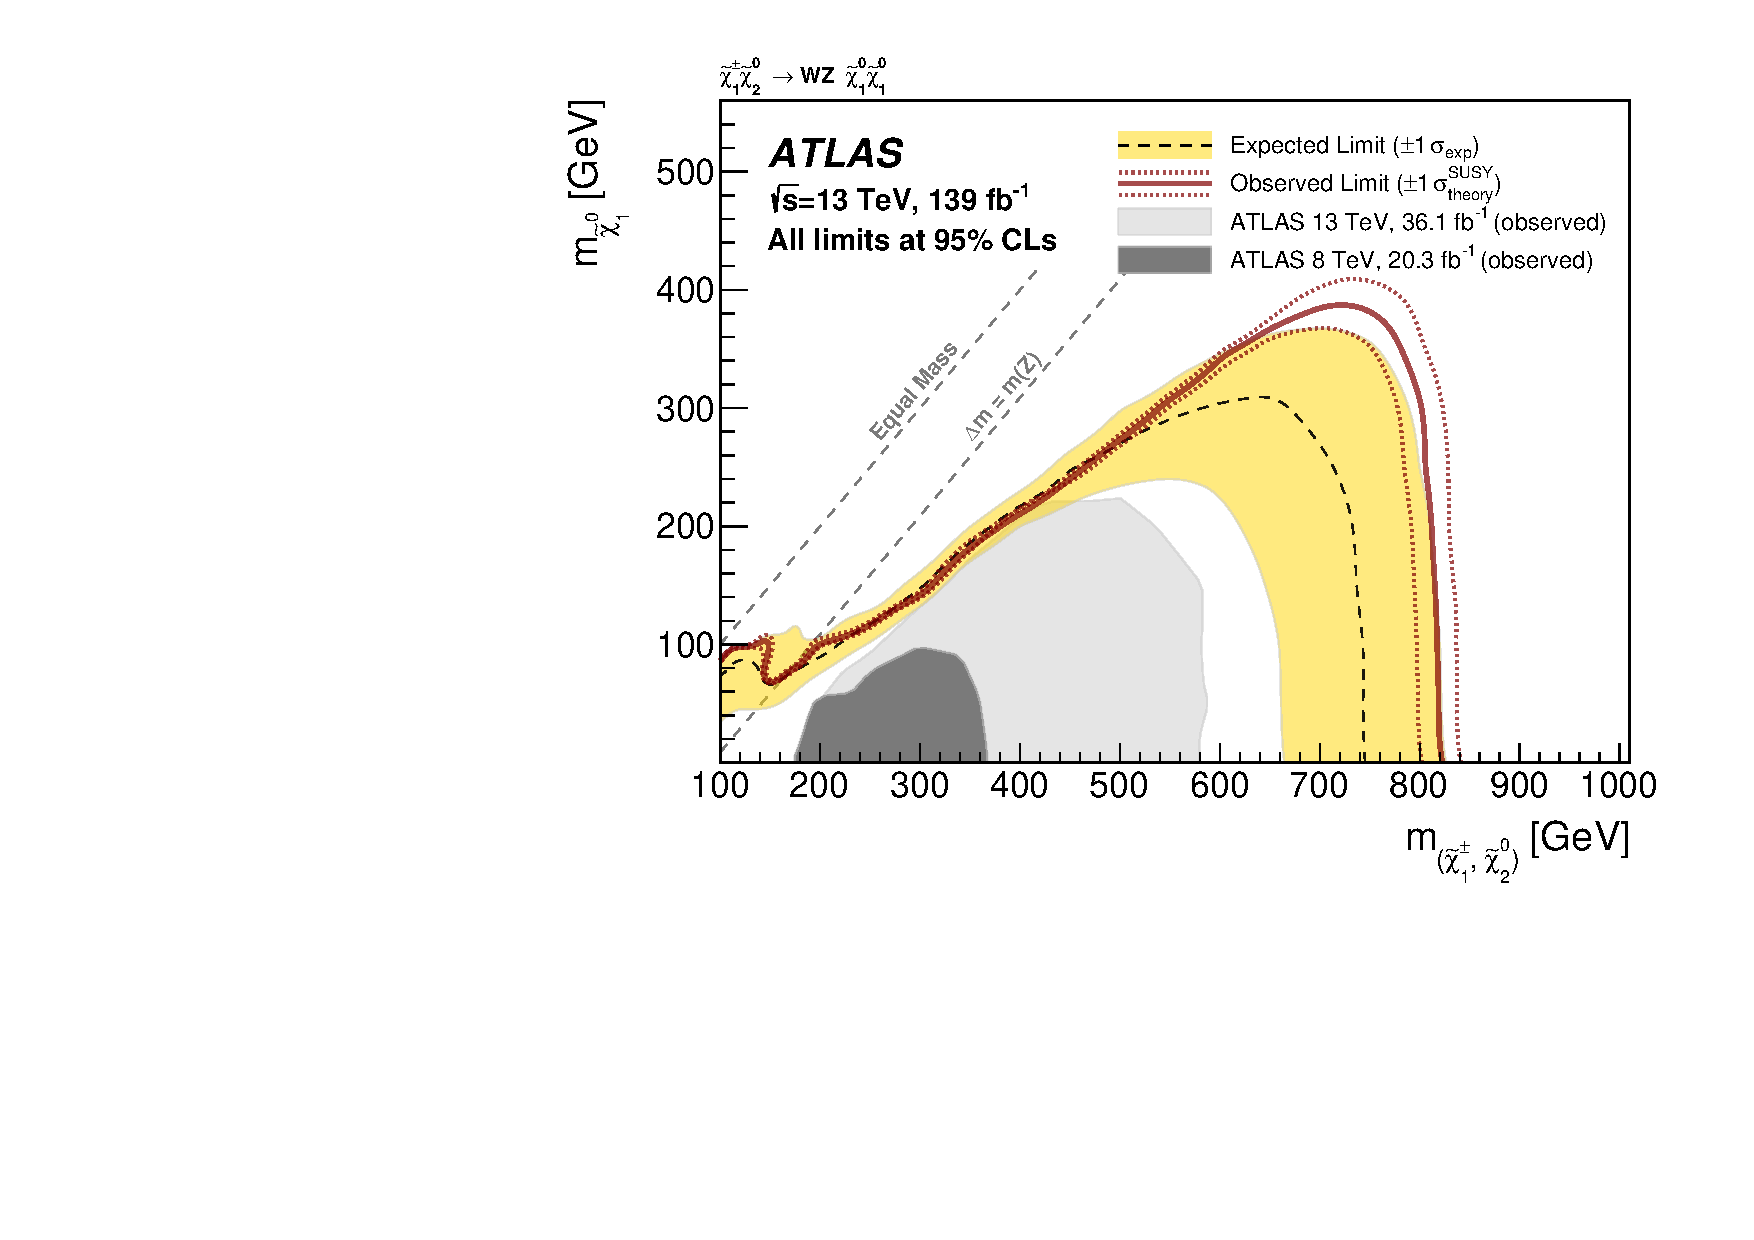
\includegraphics[width=0.99\textwidth]{figures/2ljets_contours_c1n2.pdf}
\caption{%
Contours for the C1N2 model in the $\twoljets$ electroweak
analysis~\cite{atlas2022searches}.
\\[0.5em]
Space below the solid red line is labelled as excluded and its dotted
neighbours show the result if all signal cross-sections are varied up and down
by theoretical error bars.
\\[0.5em]
The yellow band shows the $\pm1$-sigma region of exclusion contours
from asymptotic approximations to the prior distribution of the test statistic.
Grey areas are observed limits from the two-lepton parts
of~\cite{atlas_23l_SUSY_2016_24} and~\cite{atlas_2l_SUSY_2013_11}.
Exclusion is defined by the $95\%$ $\mathrm{CLs}$ prescription
in asymptotic approximations.
All contours are interpolated from a sparse grid.
}
\label{fig:2ljets_contours_c1n2}
\end{figure}

\begin{figure}[tp]
\centering
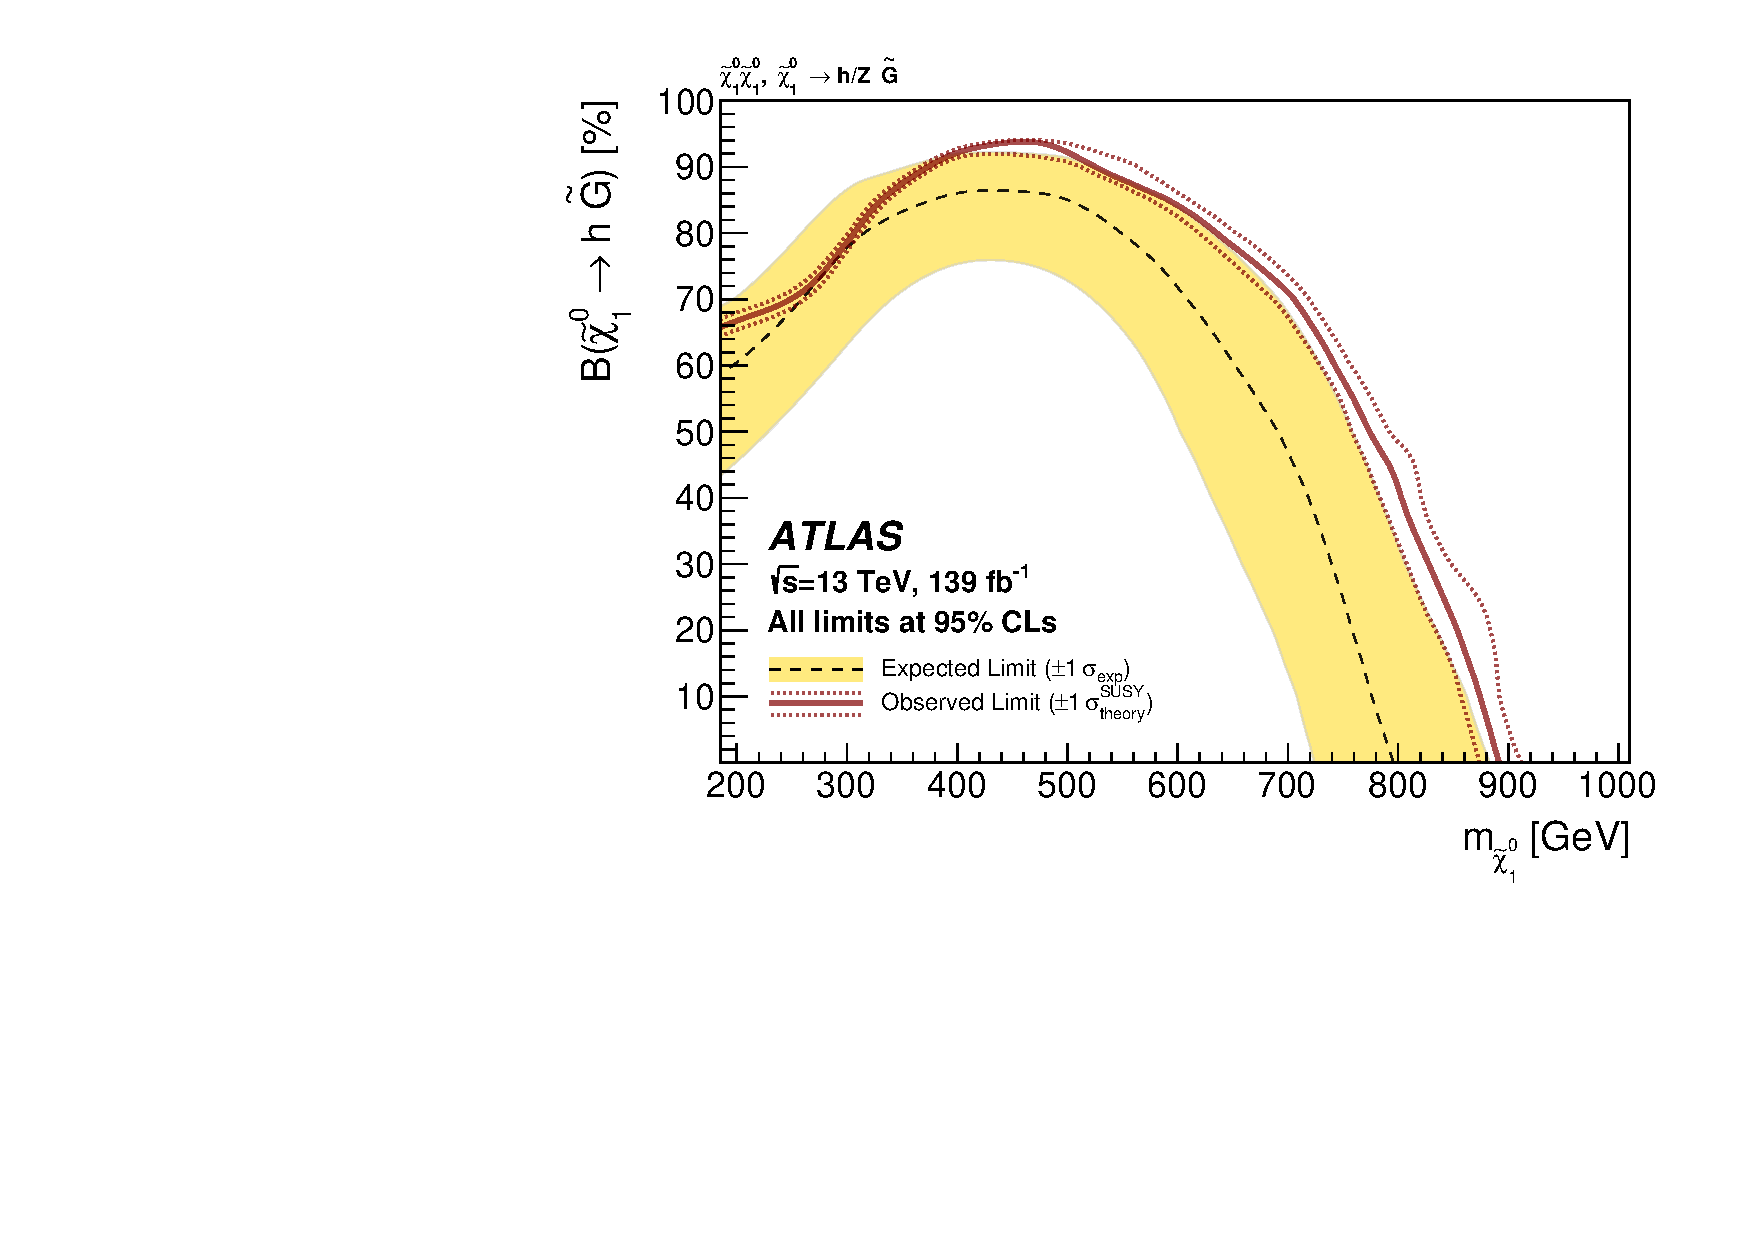
\includegraphics[width=0.99\textwidth]{figures/2ljets_contours_gmsb.pdf}
\caption{%
Contours for the GMSB model in the $\twoljets$ electroweak
analysis~\cite{atlas2022searches}.
\\[0.5em]
Space below the solid red line is labelled as excluded and its dotted
neighbours show the result if all signal cross-sections are varied up and down
by theoretical error bars.
\\[0.5em]
The yellow band shows the $\pm1$-sigma region of exclusion contours
from asymptotic approximations to the prior distribution of the test statistic.
Exclusion is defined by the $95\%$ $\mathrm{CLs}$ prescription
in asymptotic approximations.
All contours are interpolated from a sparse grid.
}
\label{fig:2ljets_contours_gmsb}
\end{figure}


% upper limits
% definitely want this after pictures
\FloatBarrier
\begin{table}[tp]
\centering
% custom separator for aligned +-
% https://stackoverflow.com/a/2132998
\begin{tabular*}{\textwidth}{lr@{$~\pm~$}lccrrcc}
Region &
\multicolumn{2}{c}{Fitted} &
Data &
$\langle A\epsilon{ \sigma}\rangle_{\mathrm{obs}}^{95}~\mathrm{fb}$ &
$S_{\mathrm{obs}}^{95}$  &
$S_{\mathrm{exp}}^{95}$ &
$\mathrm{CLb}$ &
$p(s=0)$  \\[1.5ex]
DR-OffShell      & $22.1$ & $2.7$ & 21 & $0.10$ & $14.3$ & $12.3^{+4.7}_{-3.1}$ & $0.68$ & $0.50$ \\[.5ex]
DR-Low           & $22$ & $4$ & 18 & $0.08$ & $10.8$ & $15.3^{+5.7}_{-4.0}$ & $0.09$ & $0.50$ \\[.5ex]
DR-Int           & $35$ & $4$ & 38 & $0.15$ & $20.9$ & $17.5^{+5.9}_{-3.9}$ & $0.73$ & $0.23$ \\[.5ex]
DR-High          & $3.9$ & $0.5$  & 0  & $0.02$ & $3.0$ & $5.6^{+2.2}_{-1.5}$ & $0.00$ & $0.50$ \\[.5ex]
DR-$\ell\ell bb$ & $0.51$ & $0.20$  & 0  & $0.02$ & $3.0$ & $3.0^{+1.3}_{-0.0}$ & $0.19$ & $0.50$ \\[.5ex]
\end{tabular*}
\caption{%
Upper limit results in $\twoljets$ electroweak discovery
regions~\cite{atlas2022searches}.
The fitted yield is in the background-only model constrained by the data in each region.
Limits are intended to reflect constrains on additive signal contributions.
\\[0.5em]
Left to right:
the region name,
the post-fit background expectation,
the number of data observed,
the observed $95\%$ $\mathrm{CLs}$ upper limit on the visible cross-section
$\langle\epsilon\sigma\rangle_\mathrm{obs}^{95}$,
its corresponding signal expectation $S_\mathrm{obs}^{95}$,
the expected $95\%$ upper limits on the signal expectation $S_\mathrm{exp}^{95}$
as would be obtained were the test statistic given by its central or
$\pm1$-sigma variations,
$\mathrm{CLb}$ evaluated with the signal expectation set to the observed upper limit,
and the discovery $p$-value (capped at $0.5$) with its equivalent significance.
\\[0.5em]
Upper limits use the one-sided profile likelihood test statistic.
The discovery $p$-value uses a profile likelihood test statistic in a one-sided test.
All $p$-values are estimated by simulation of alternative data.
\TODO{add labels and references to asymptotic formulae paper}
\TODO{reference pdg rounding}
}
\label{tab:2ljets_discovery}
\end{table}

\FloatBarrier
\subsection{Contributions}

This subsection claims attributions of work on the $\twoljets$ analysis.

\begin{itemize}
\item Design, implementation and execution of the electroweak part of the analysis.
\item Service as `analysis contact' from January to October 2020.
\item Production of main data inputs for all three analyses
and the RJR $3\ell$ search \TODO{cite}.
Production of all systematic variations for the background samples;
other group members assisted with the central background sample.
Production of all electroweak signal samples and their systematic variations.
\item Integration with ATLAS combinations and pMSSM scan efforts by
performing their validation studies and serializing the analysis results.
\item Preparation of electroweak results for publication in the paper \TODO{cite} and the
public HEPData record~\cite{maguire2017hepdata}.
\end{itemize}
Except where specified, I produced all figures presented in this thesis.
Many plotting scripts, however, are modified from versions inherited from
many \atlas\ members past and present to whom I am grateful.

Of the large collaboration involved in this project, a great deal of credit is
due to the following colleagues, labelled with their primary focus within
the $\twoljets$ search effort:
Knut Oddvar Vadla (electroweak),
Sarah Williams (electroweak),
Jason Lea Oliver (RJR),
Abhishek Sharma (RJR),
Jonathan Long (strong),
Arka Santra (strong),
Matt Zhang (strong),
Yumeng Cao (various),
Eirik Gramstad (fake/non-prompt leptons),
Benjamin Henry Hooberman (leadership).
Cheers.

\clearpage
\FloatBarrier
\section{Context}
\label{sec:2ljets_context}
% previous results on 2(/3)L from ATLAS
% other constraints on these models from ATLAS/CMS
% previous region design, motivation for this work
Previous analyses of \atlas\ data have explored similar selections of
two leptons, jets, and missing transverse momentum.
Quite a few analyses, in fact.
This project exists to supplement those results with information from the full
LHC Run 2 data-set which was completed in 2018 and contains
$139~\mathrm{fb}^{-1}$ of usable proton-proton collisions at $\sqrt{s} = 13~\eV[T]$.
Leverage of the increased data quantity is one key aim.
Analysis quality also might be improved if our designs can take lessons from
the experiences of previous work.

% electroweak
% Run 1 data~\cite{atlas_2l_SUSY_2013_11},
% partial Run 2 data~\cite{atlas_23l_SUSY_2016_24},
% atlas_rjr_23l_SUSY_2017_03,
% atlas_rjr_mimic_SUSY_2018_06

The $\twoljets$ analysis is a trinity,
of which all three parts update previously published \atlas\ results.
These three parts are named `RJR', `electroweak', and `strong', each of which
is described in its historical context in this section.

Recursive Jigsaw Reconstruction (RJR) is an algorithm for constructing useful
event variables.
The $\twoljets$ RJR analysis, detailed in Section~\ref{sec:2ljets_origins_rjr},
uses RJR variables to define its regions in a signal-independent search.

My primary contributions are to the $\twoljets$ electroweak analysis,
detailed in Section~\ref{sec:2ljets_origins_electroweak},
which uses conventional (non-RJR) event variables to define a collection of
orthogonal regions, and performs a search for effects from the electroweak
sectors of supersymmetric models.

Unsurprisingly, the strong part of the $\twoljets$ analysis is
detailed in Section~\ref{sec:2ljets_origins_strong} and
searches for effects from the strong sector.
It also uses conventional event variables, and focuses on features in the
distribution of the invariant masses of lepton pairs.


\subsection{RJR}
\label{sec:2ljets_origins_rjr}

\begin{figure}[tp]
\centering
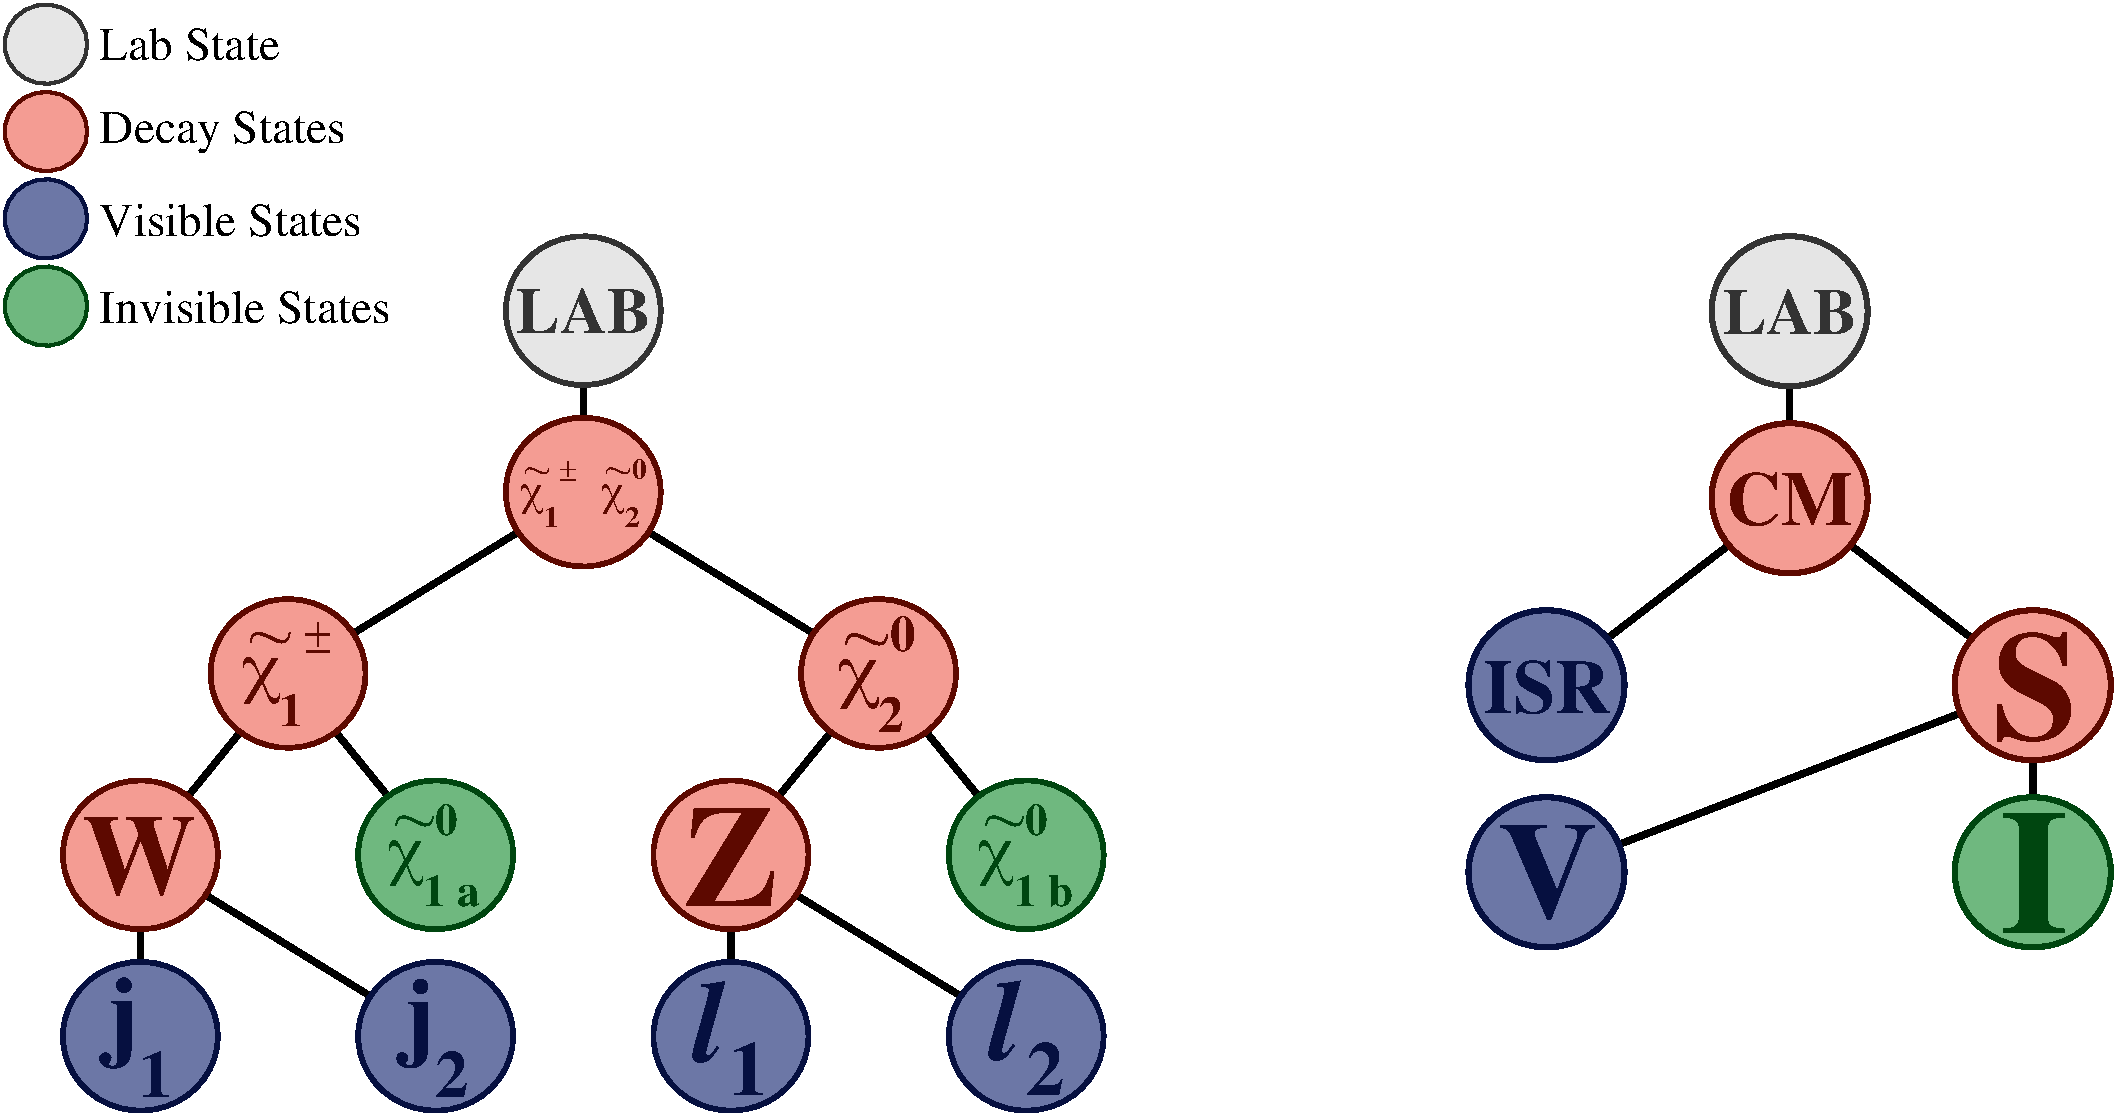
\includegraphics[width=0.9\textwidth]{figures/2ljets_rjr_trees.pdf}
\caption{%
Decay trees for the $\twoljets$ RJR analysis~\cite{atlas2022searches}.
Both diagrams represent processes also targetted in the electroweak analysis.
(left) A fully-resolved decay tree with its particles labelled.
(right) Only the $Z\rightarrow\ell\ell$ (\underline{V}ector boson)
is resolved, but the supersymmetric system recoils off
hard QCD jets labelled ``ISR'', boosting the \underline{I}nvisible particles,
to generate visibly large $\met$ in models with small mass-splittings.
The same approach is used for SR-OffShell selections in the electroweak
analysis.
\emph{This figure was made by the RJR team.}
}
\label{fig:2ljets_rjr_decay_trees}
\end{figure}

The Recursive Jigsaw Reconstruction (RJR) method interprets reconstructed
particle data by reconciling them with user-specified decay trees, and works
by making decisions of how to assign four-momenta to different `systems',
which are nodes of the chosen the decay graph.
Event variables are then evaluated in those systems' rest
frames~\cite{jackson2017sparticles, jackson2017rjr}.

In this way, RJR variables get some intelligence in how parent particles are
reconstructed from their visible decay products, as well as approximate
independence from uninteresting boosts, particularly those from the emission of
QCD jets outside of the supersymmetric decay tree.

Over the last several years, RJR event variables have been demonstrated to be
effective for interpreting supersymmetric particle physics
data~\cite{santoni2018probing},
and have been used in numerous \atlas\ analyses~\cite{%
atlas_rjr_SUSY_2016_07,
atlas_rjr_SUSY_2016_15,
atlas_rjr_SUSY_2016_16,
atlas_rjr_23l_SUSY_2017_03,
atlas_rjr_3l_SUSY_2019_09
} \TODO{more}.
They have also influenced the designs of other analyses which do not use
RJR variables themselves~\cite{atlas_rjr_mimic_SUSY_2018_06}.


Two decay trees are used in the $\twoljets$ RJR analysis, with signal region
each.
These trees target C1N2-like scenarios similar to those also considered in the
$\twoljets$ electroweak search,
and illustrated in Figure~\ref{fig:2ljets_rjr_decay_trees}.

\paragraph{Former excesses}
Excess data were observed in several signal regions of the partial Run 2
search ``for chargino--neutralino production using recursive
jigsaw reconstruction in final states with two or three charged
leptons''~\cite{atlas_rjr_23l_SUSY_2017_03},
which used $36.1~\mathrm{fb}^{-1}$ of proton-proton collisions at
$\sqrt{s} = 13~\eV[T]$.
That search reported notable excesses in four signal regions.
Of these, two required two charged leptons
($\mathrm{SR}2\ell\_\mathrm{Low}$ and $\mathrm{SR}2\ell\_\mathrm{ISR}$),
and other two required three
($\mathrm{SR}3\ell\_\mathrm{Low}$ and $\mathrm{SR}3\ell\_\mathrm{ISR}$).

Although the largest local excess was reported as ``$3.0$ standard deviations'',
which is not particularly large, the pattern of four related regions with
excess data can understandably draw attention.

Both $\mathrm{SR}3\ell\_\mathrm{Low}$ and $\mathrm{SR}3\ell\_\mathrm{ISR}$
were have been revisited with the full Run 2 data-set and updated background
modelling.
The update sees ``no significant excesses''~\cite{atlas_rjr_3l_SUSY_2019_09}.
These regions have also been approximated without direct use of RJR event
variables;
these approximations also find data ``in agreement'' with the background
model~\cite{atlas_rjr_mimic_SUSY_2018_06}.

The $\twoljets$ RJR serves to analysis reproduce
$\mathrm{SR}2\ell\_\mathrm{Low}$ and $\mathrm{SR}2\ell\_\mathrm{ISR}$,
with the full Run 2 data-set and updated background modelling,
and asks whether the excesses persist.
They do not.

\paragraph{Versus conventional}
Disappearing excesses have encouraged doubts about RJR variables;
the existence of the `RJR-mimic' paper~\cite{atlas_rjr_mimic_SUSY_2018_06}
is public evidence of this.

A more precise problem is that that phase space selected by RJR regions tends
to be poorly (inaccurately or imprecisely) modelled by simulations.
This is plausibly explained how RJR variables are not simply related to
conventional, lab-frame variables.
Simulations have been tuned to model conventional variables well, and
`systematic' variations also are evaluated and derived in conventional variables.
Not all functions of the data are well understood.

A lack of reliable simulations motivates reliance on `data-driven' background
estimates, which, from my perspective, are hard to interpret or trust.
For these reasons, the $\twoljets$ electroweak analysis uses only conventional
event variables.

\subsection{Electroweak}
\label{sec:2ljets_origins_electroweak}

\subsection{Strong}
\label{sec:2ljets_origins_strong}


\section{Event variables}
% lepton, jet definitions


\subsection{$\met$ significance}
\label{sec:metsig}
It scales $\met$ by an uncertainty derived from the resolutions of
reconstructed objects~\cite{atlas_met_significance}.

\subsection{Stranverse mass $\mttwo$}
\label{sec:mt2}
% angle between the vector sum of the lepton pair and the missing transverse momentum.
% leptons and the missing transverse momentum.
% If two massive particles are pair produced and each decays to a
% lepton and something massless and invisible,
% then this estimates a greatest lower bound on the invariant
% mass of the pair produced particles.
% $\mttwo(\ell, \ell; 0)$ is useful for excluding standard model backgrounds;
% di-leptonic ttbar ($tt\rightarrow WW\rightarrow\ell\nu\ell\nu$)
% and $WW\rightarrow\ell\nu\ell\nu$ have a kinematic endpoint
% at the $W$ pole mass, and $\tau\tau$ is constrained within measurement error of zero.

\subsection{$b$-tagging}
\label{sec:btagging}
% with $\pt > 20$ GeV,
% where the tag is taken on the mv2c10 classifier at the $77\%$ working point.

\subsection{Cheat-sheet}
Uncomfortably many event variables are used to define the regions of this
analysis.
To aid future revision of their meanings, definitions and references for these
variables are collected here.
\begin{itemize}
\item $\met$: missing transverse momentum
\item $\metsig$: object-based missing transverse momentum significance;\\
described in Section~\ref{sec:metsig}
\item $\ptjone$: transverse momentum of the hardest jet%
\vspace{0.5em}
\item $\mll$: invariant mass of the hardest two leptons
\item $\mjj$: invariant mass of the two hardest jets
\item $\mbb$: invariant mass of the two hardest b-tagged jets
\item $\mjetone$: mass of the hardest jet
\item $\mttwoll$: `stransverse` mass of the lepton pair with massless invisibles;\\
described in Section~\ref{sec:mt2}
\vspace{0.5em}
\item $\rll$: distance in $\eta\textrm{--}\phi$ between the lepton pair
\item $\rjj$: distance in $\eta\textrm{--}\phi$ between the two hardest jets%
\vspace{0.5em}
\item $n_{\mathrm{jets},30}$: number of reconstructed jets with $\pt > 30$ GeV.
\item $\nbtag$: number of b-tagged jets;
described in Section~\ref{sec:btagging}
\vspace{0.5em}
\item $\dphillmet$: azimuthal angle between the hardest jet and $\ptmiss$
\item $\Delta\phi(\mathrm{jet}_1,\met)$: azimuthal angle between
the hardest jet and $\ptmiss$
\end{itemize}
All of these are physical properties of particles or collections of particles.
Please remember that none is an exact or true value;
all are are estimates based on approximate reconstructions.
While this distinction is easy to drop in lax language, is necessary to
understand the shapes of noisy variables such as $\mjj$ and indeed the
existence of $\metsig$.

\FloatBarrier
\section{Design}

The most impactful decision in a search is the design of its regions.
Like all decision in life, these designs must be made to balance conflicting
and vaguely-specified desires, and are informed with incomplete information.

This section describes the designs and rationales behind the control, validation
and signal regions of the $\twoljets$ analysis.


Splitting regions on $\metsig$ is the core idea behind the design.
The basic motivation for this design are displayed in
Figure~\ref{fig:2ljets_presel_met};
$\metsig$ does better than $\met$ in separating background and signal
contributions.
But there is more --- $\metsig$ also does a decent job of separating signal
models from each other;
signals with larger mass differences in their decays to invisibles tend to have
larger $\metsig$.
Binning regions in $\metsig$ therefore also improves sensitivity to
individual parameter points and allows targeted selections on other, locally-relevant,
event variables.

\begin{figure}[tp]
\centering
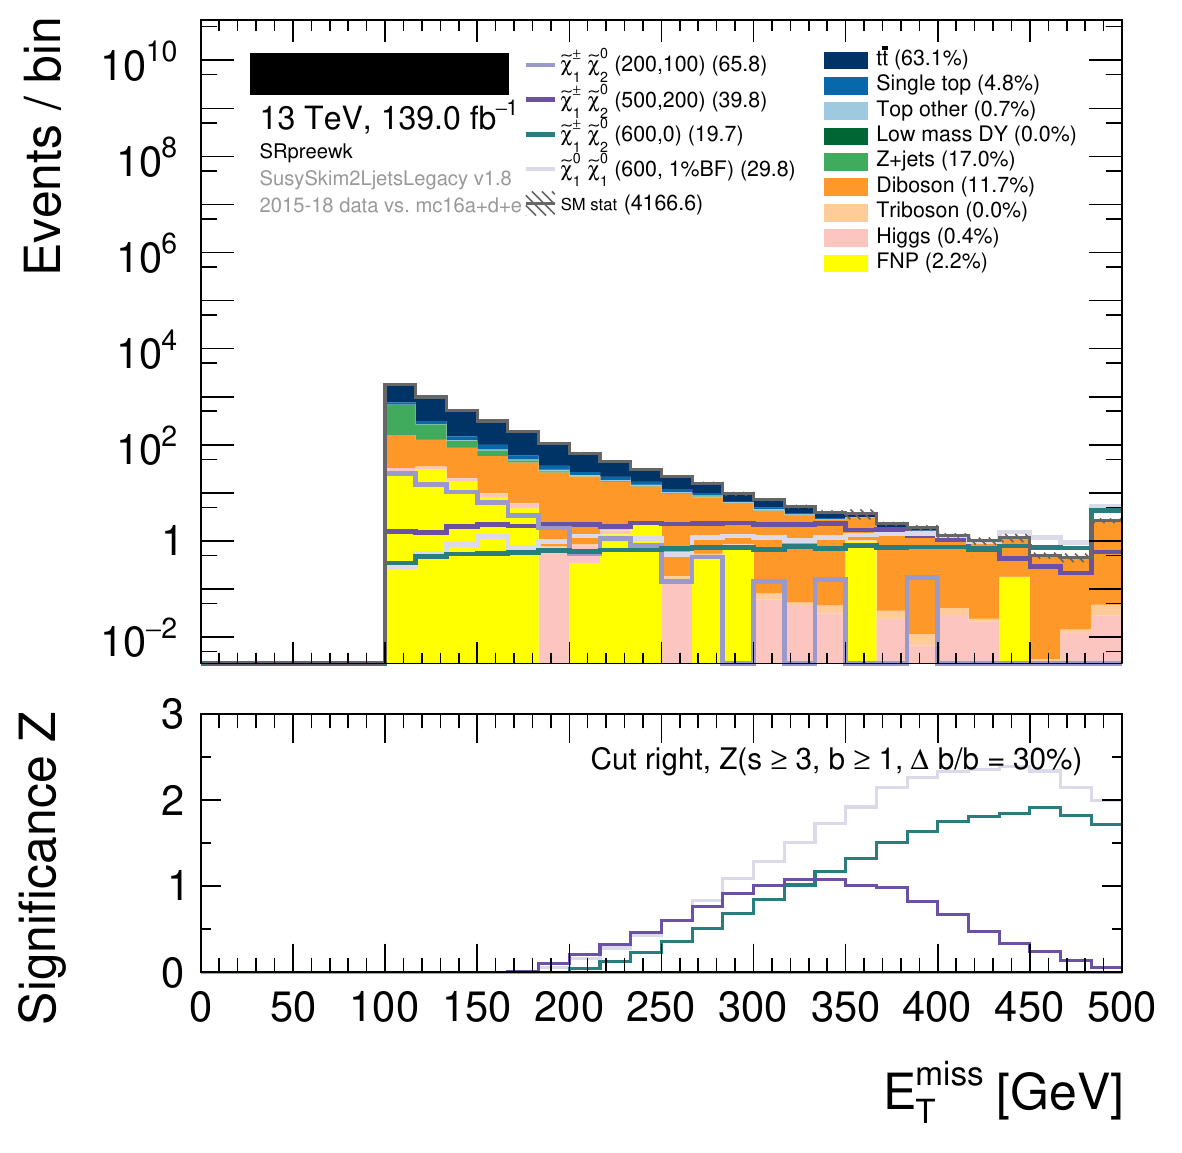
\includegraphics[width=0.49\textwidth]{figures/2ljets_presel_met_logy.png}
\hfill
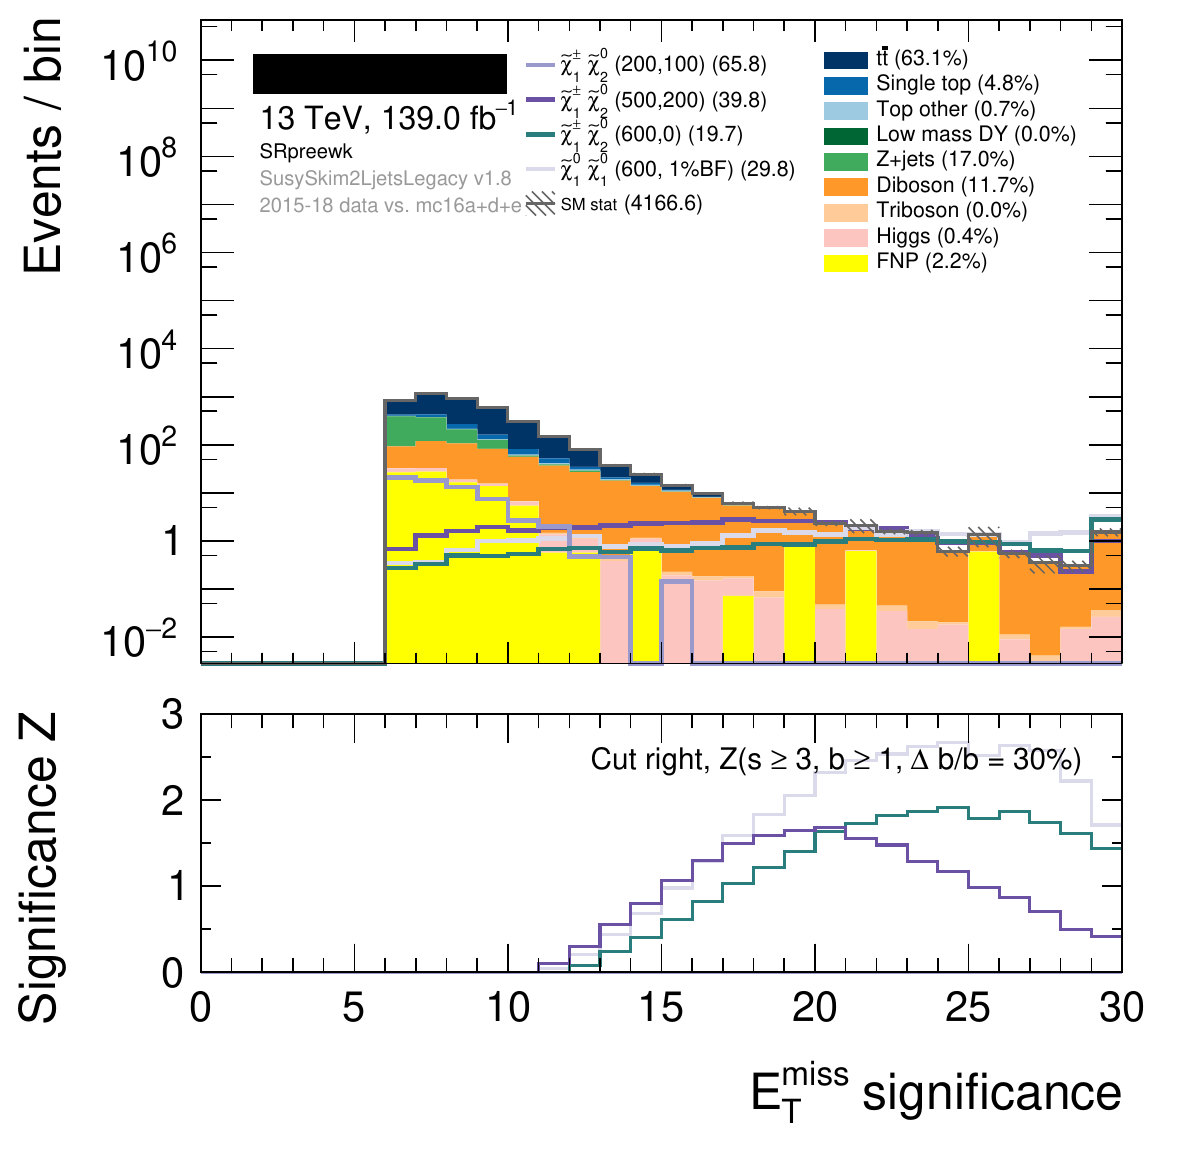
\includegraphics[width=0.49\textwidth]{figures/2ljets_presel_met_sig_logy.png}
\caption{
Illustration of how $\metsig$ beats $\met$ alone in sensitivity to
example signal models.
At large $\metsig$, $t\bar t$ and other backgrounds are suppressed, leaving
quite pure diboson backgrounds and greater significance measures.
Signal models with smaller mass splittings tend to have the bulk of their
events at smaller $\met$.
\\[0.5em]
This loose selection ``SRpreewk'' requires two same-flavor opposite-sign
signal leptons with
$\mll \in (71, 111)~\eV[G]$,
$\mjj \in (60, 110)~\eV[G]$,
$\nbtag \leq 1$,
$\met > 100~\eV[G]$, and
$\metsig > 6$.
\\[0.5em]
``Significance'' displayed in the lower subplot uses the Binomial significance
$Z_{Bi}$ from~\cite{cousins2008evaluation}, with a $30\%$ background
uncertainty and yields taken to the right of a given value.
Large values indicate expected sensitivity to the signal model.
}
\label{fig:2ljets_presel_met}
\end{figure}



% CRs go in with relevant SR category
\subsection{High}

\subsection{Intermediate}

\subsection{Low}

\subsection{Off-shell}

\subsection{Discovery}

\section{Modelling}
% TODO backgorund samples
% TODO matrix method fakes
% TODO GMSB reweighting
% TODO off-shell plus/minus split
% TODO generator filtering

\subsection{Fake/non-prompt leptons}

\section{Validation}

\section{Systematics}

\section{Results}


